\clearpage

\section{Pre-Supernova Abundance}
While nucleosynthesis takes place throughout a star's lifetime, this section focuses on the final abundance profiles at core collapse. Mass fraction and yield plots are presented for key isotopes—$^{12}$C, $^{14}$N, and $^{16}$O—across our model grid, which spans different metallicities and CBM rates. These final-stage abundance patterns encapsulate the cumulative effects of nuclear network selection, metallicity, and mixing processes on stellar evolution, and they provide critical insight into the chemical yields that contribute to the enrichment of the interstellar medium.

%–––––––––––––––––––––––––––––––––––––––
%12C_YIELDS_AND_MASS_FRACTIONS
%–––––––––––––––––––––––––––––––––––––––

\subsection{$^{12}$C Yields and Mass Fractions}

%15M_5CBM
\begin{minipage}{\textwidth}
	\centering
	\begin{subfigure}{0.49\textwidth}
		\includegraphics[width=\textwidth]{12C_Mass_Fracs/15M/M12C vs Mr Z_Comparison at 5CBM.png}
	\end{subfigure}
        \hfill
	\begin{subfigure}{0.49\textwidth}
		\includegraphics[width=\textwidth]{12C_Mass_Fracs/15M/X12C vs Mr Z_Comparison at 5CBM.png}
	\end{subfigure}
        \label{fig:12C_15M_5CBM}
\end{minipage}
%15M_2CBM
\begin{minipage}{\textwidth}
	\centering
	\begin{subfigure}{0.49\textwidth}
		\includegraphics[width=\textwidth]{12C_Mass_Fracs/15M/M12C vs Mr Z_Comparison at 2CBM.png}
	\end{subfigure}
        \hfill
	\begin{subfigure}{0.49\textwidth}
		\includegraphics[width=\textwidth]{12C_Mass_Fracs/15M/X12C vs Mr Z_Comparison at 2CBM.png}
	\end{subfigure}
        \label{fig:12C_15M_2CBM}
\end{minipage}
%15M_0.5CBM
\begin{minipage}{\textwidth}
	\centering
	\begin{subfigure}{0.49\textwidth}
		\includegraphics[width=\textwidth]{12C_Mass_Fracs/15M/M12C vs Mr Z_Comparison at 0.5CBM.png}
	\end{subfigure}
        \hfill
	\begin{subfigure}{0.49\textwidth}
		\includegraphics[width=\textwidth]{12C_Mass_Fracs/15M/X12C vs Mr Z_Comparison at 0.5CBM.png}
	\end{subfigure}
	 \caption{Comparison of $^{12}$C Mass Yield (left) and Mass Fraction (right) for a 15M$_\odot$ model at various metallicities, categorised by CBM Rates.}
        \label{fig:12C_15M_0.5CBM}
\end{minipage}

%20M_5CBM
\begin{minipage}{\textwidth}
	\centering
	\begin{subfigure}{0.49\textwidth}
		\includegraphics[width=\textwidth]{12C_Mass_Fracs/20M/M12C vs Mr Z_Comparison at 5CBM.png}
	\end{subfigure}
        \hfill
	\begin{subfigure}{0.49\textwidth}
		\includegraphics[width=\textwidth]{12C_Mass_Fracs/20M/X12C vs Mr Z_Comparison at 5CBM.png}
	\end{subfigure}
        \label{fig:12C_20M_5CBM}
\end{minipage}
%20M_2CBM
\begin{minipage}{\textwidth}
	\centering
	\begin{subfigure}{0.49\textwidth}
		\includegraphics[width=\textwidth]{12C_Mass_Fracs/20M/M12C vs Mr Z_Comparison at 2CBM.png}
	\end{subfigure}
        \hfill
	\begin{subfigure}{0.49\textwidth}
		\includegraphics[width=\textwidth]{12C_Mass_Fracs/20M/X12C vs Mr Z_Comparison at 2CBM.png}
	\end{subfigure}
        \label{fig:12C_20M_2CBM}
\end{minipage}
%20M_0.5CBM
\begin{minipage}{\textwidth}
	\centering
	\begin{subfigure}{0.49\textwidth}
		\includegraphics[width=\textwidth]{12C_Mass_Fracs/25M/M12C vs Mr Z_Comparison at 0.5CBM.png}
	\end{subfigure}
        \hfill
	\begin{subfigure}{0.49\textwidth}
		\includegraphics[width=\textwidth]{12C_Mass_Fracs/25M/X12C vs Mr Z_Comparison at 0.5CBM.png}
	\end{subfigure}
	 \caption{Comparison of $^{12}$C Mass Yield (left) and Mass Fraction (right) for a 20M$_\odot$ model at various metallicities, categorised by CBM Rates.}
        \label{fig:12C_20M_0.5CBM}
\end{minipage}

%25M_5CBM
\vspace{1em}
\begin{minipage}{\textwidth}
	\centering
	\begin{subfigure}{0.49\textwidth}
		\includegraphics[width=\textwidth]{12C_Mass_Fracs/25M/M12C vs Mr Z_Comparison at 5CBM.png}
	\end{subfigure}
        \hfill
	\begin{subfigure}{0.49\textwidth}
		\includegraphics[width=\textwidth]{12C_Mass_Fracs/25M/X12C vs Mr Z_Comparison at 5CBM.png}
	\end{subfigure}
        \label{fig:12C_25M_5CBM}
\end{minipage}
%25M_2CBM
\begin{minipage}{\textwidth}
	\centering
	\begin{subfigure}{0.49\textwidth}
		\includegraphics[width=\textwidth]{12C_Mass_Fracs/25M/M12C vs Mr Z_Comparison at 2CBM.png}
	\end{subfigure}
        \hfill
	\begin{subfigure}{0.49\textwidth}
		\includegraphics[width=\textwidth]{12C_Mass_Fracs/25M/X12C vs Mr Z_Comparison at 2CBM.png}
	\end{subfigure}
        \label{fig:12C_25M_2CBM}
\end{minipage}
%25M_0.5CBM
\begin{minipage}{\textwidth}
	\centering
	\begin{subfigure}{0.49\textwidth}
		\includegraphics[width=\textwidth]{12C_Mass_Fracs/25M/M12C vs Mr Z_Comparison at 0.5CBM.png}
	\end{subfigure}
        \hfill
	\begin{subfigure}{0.49\textwidth}
		\includegraphics[width=\textwidth]{12C_Mass_Fracs/25M/X12C vs Mr Z_Comparison at 0.5CBM.png}
	\end{subfigure}
	 \caption{Comparison of $^{12}$C Mass Yield (left) and Mass Fraction (right) for a 25M$_\odot$ model at various metallicities, categorised by CBM Rates.}
        \label{fig:12C_25M_0.5CBM}
\end{minipage}

%–––––––––––––––––––––––––––––––––––––––
%14N_YIELDS_AND_MASS_FRACTIONS
%–––––––––––––––––––––––––––––––––––––––

\subsection{$^{14}$N Yields and Mass Fractions}
%15M_5CBM
\begin{minipage}{\textwidth}
	\centering
	\begin{subfigure}{0.49\textwidth}
		\includegraphics[width=\textwidth]{14N_Mass_Fracs/15M/M14N vs Mr Z_Comparison at 5CBM.png}
	\end{subfigure}
        \hfill
	\begin{subfigure}{0.49\textwidth}
		\includegraphics[width=\textwidth]{14N_Mass_Fracs/15M/X14N vs Mr Z_Comparison at 5CBM.png}
	\end{subfigure}
        \label{fig:14N_15M_5CBM}
\end{minipage}
%15M_2CBM
\begin{minipage}{\textwidth}
	\centering
	\begin{subfigure}{0.49\textwidth}
		\includegraphics[width=\textwidth]{14N_Mass_Fracs/15M/M14N vs Mr Z_Comparison at 2CBM.png}
	\end{subfigure}
        \hfill
	\begin{subfigure}{0.49\textwidth}
		\includegraphics[width=\textwidth]{14N_Mass_Fracs/15M/X14N vs Mr Z_Comparison at 2CBM.png}
	\end{subfigure}
        \label{fig:14N_15M_2CBM}
\end{minipage}
%15M_0.5CBM
\begin{minipage}{\textwidth}
	\centering
	\begin{subfigure}{0.49\textwidth}
		\includegraphics[width=\textwidth]{14N_Mass_Fracs/15M/M14N vs Mr Z_Comparison at 0.5CBM.png}
	\end{subfigure}
        \hfill
	\begin{subfigure}{0.49\textwidth}
		\includegraphics[width=\textwidth]{14N_Mass_Fracs/15M/X14N vs Mr Z_Comparison at 0.5CBM.png}
	\end{subfigure}
	 \caption{Comparison of $^{14}$N Mass Yield (left) and Mass Fraction (right) for a 15M$_\odot$ model at various metallicities, categorised by CBM Rates.}
        \label{fig:14N_15M_0.5CBM}
\end{minipage}

%20M_5CBM
\begin{minipage}{\textwidth}
	\centering
	\begin{subfigure}{0.49\textwidth}
		\includegraphics[width=\textwidth]{14N_Mass_Fracs/20M/M14N vs Mr Z_Comparison at 5CBM.png}
	\end{subfigure}
        \hfill
	\begin{subfigure}{0.49\textwidth}
		\includegraphics[width=\textwidth]{14N_Mass_Fracs/20M/X14N vs Mr Z_Comparison at 5CBM.png}
	\end{subfigure}
        \label{fig:14N_20M_5CBM}
\end{minipage}
%20M_2CBM
\begin{minipage}{\textwidth}
	\centering
	\begin{subfigure}{0.49\textwidth}
		\includegraphics[width=\textwidth]{14N_Mass_Fracs/20M/M14N vs Mr Z_Comparison at 2CBM.png}
	\end{subfigure}
        \hfill
	\begin{subfigure}{0.49\textwidth}
		\includegraphics[width=\textwidth]{14N_Mass_Fracs/20M/X14N vs Mr Z_Comparison at 2CBM.png}
	\end{subfigure}
        \label{fig:14N_20M_2CBM}
\end{minipage}
%20M_0.5CBM
\begin{minipage}{\textwidth}
	\centering
	\begin{subfigure}{0.49\textwidth}
		\includegraphics[width=\textwidth]{14N_Mass_Fracs/20M/M14N vs Mr Z_Comparison at 0.5CBM.png}
	\end{subfigure}
        \hfill
	\begin{subfigure}{0.49\textwidth}
		\includegraphics[width=\textwidth]{14N_Mass_Fracs/20M/X14N vs Mr Z_Comparison at 0.5CBM.png}
	\end{subfigure}
	 \caption{Comparison of $^{14}$N Mass Yield (left) and Mass Fraction (right) for a 20M$_\odot$ model at various metallicities, categorised by CBM Rates.}
        \label{fig:14N_20M_0.5CBM}
\end{minipage}

%25M_5CBM
\begin{minipage}{\textwidth}
	\centering
	\begin{subfigure}{0.49\textwidth}
		\includegraphics[width=\textwidth]{14N_Mass_Fracs/25M/M14N vs Mr Z_Comparison at 5CBM.png}
	\end{subfigure}
        \hfill
	\begin{subfigure}{0.49\textwidth}
		\includegraphics[width=\textwidth]{14N_Mass_Fracs/25M/X14N vs Mr Z_Comparison at 5CBM.png}
	\end{subfigure}
        \label{fig:14N_25M_5CBM}
\end{minipage}
%25M_2CBM
\begin{minipage}{\textwidth}
	\centering
	\begin{subfigure}{0.49\textwidth}
		\includegraphics[width=\textwidth]{14N_Mass_Fracs/25M/M14N vs Mr Z_Comparison at 2CBM.png}
	\end{subfigure}
        \hfill
	\begin{subfigure}{0.49\textwidth}
		\includegraphics[width=\textwidth]{14N_Mass_Fracs/25M/X14N vs Mr Z_Comparison at 2CBM.png}
	\end{subfigure}
        \label{fig:14N_25M_2CBM}
\end{minipage}
%25M_0.5CBM
\begin{minipage}{\textwidth}
	\centering
	\begin{subfigure}{0.49\textwidth}
		\includegraphics[width=\textwidth]{14N_Mass_Fracs/25M/M14N vs Mr Z_Comparison at 0.5CBM.png}
	\end{subfigure}
        \hfill
	\begin{subfigure}{0.49\textwidth}
		\includegraphics[width=\textwidth]{14N_Mass_Fracs/25M/X14N vs Mr Z_Comparison at 0.5CBM.png}
	\end{subfigure}
	 \caption{Comparison of $^{14}$N Mass Yield (left) and Mass Fraction (right) for a 25M$_\odot$ model at various metallicities, categorised by CBM Rates.}
        \label{fig:14N_25M_0.5CBM}
\end{minipage}

%–––––––––––––––––––––––––––––––––––––––
%16O_YIELDS_AND_MASS_FRACTIONS
%–––––––––––––––––––––––––––––––––––––––

\subsection{$^{16}$O Yields and Mass Fractions}
%15M_5CBM
\begin{minipage}{\textwidth}
	\centering
	\begin{subfigure}{0.49\textwidth}
		\includegraphics[width=\textwidth]{16O_Mass_Fracs/15M/M16O vs Mr Z_Comparison at 5CBM.png}
	\end{subfigure}
        \hfill
	\begin{subfigure}{0.49\textwidth}
		\includegraphics[width=\textwidth]{16O_Mass_Fracs/15M/X16O vs Mr Z_Comparison at 5CBM.png}
	\end{subfigure}
        \label{fig:16O_15M_5CBM}
\end{minipage}
%15M_2CBM
\begin{minipage}{\textwidth}
	\centering
	\begin{subfigure}{0.49\textwidth}
		\includegraphics[width=\textwidth]{16O_Mass_Fracs/15M/M16O vs Mr Z_Comparison at 2CBM.png}
	\end{subfigure}
        \hfill
	\begin{subfigure}{0.49\textwidth}
		\includegraphics[width=\textwidth]{16O_Mass_Fracs/15M/X16O vs Mr Z_Comparison at 2CBM.png}
	\end{subfigure}
        \label{fig:16O_15M_5CBM}
\end{minipage}
%15M_0.5CBM
\begin{minipage}{\textwidth}
	\centering
	\begin{subfigure}{0.49\textwidth}
		\includegraphics[width=\textwidth]{16O_Mass_Fracs/15M/M16O vs Mr Z_Comparison at 0.5CBM.png}
	\end{subfigure}
        \hfill
	\begin{subfigure}{0.49\textwidth}
		\includegraphics[width=\textwidth]{16O_Mass_Fracs/15M/X16O vs Mr Z_Comparison at 0.5CBM.png}
	\end{subfigure}
	 \caption{Comparison of $^{16}$O Mass Yield (left) and Mass Fraction (right) for a 15M$_\odot$ model at various metallicities, categorised by CBM Rates.}
        \label{fig:16O_15M_0.5CBM}
\end{minipage}

%20M_5CBM
\begin{minipage}{\textwidth}
	\centering
	\begin{subfigure}{0.49\textwidth}
		\includegraphics[width=\textwidth]{16O_Mass_Fracs/20M/M16O vs Mr Z_Comparison at 5CBM.png}
	\end{subfigure}
        \hfill
	\begin{subfigure}{0.49\textwidth}
		\includegraphics[width=\textwidth]{16O_Mass_Fracs/20M/X16O vs Mr Z_Comparison at 5CBM.png}
	\end{subfigure}
        \label{fig:16O_20M_5CBM}
\end{minipage}
%20M_2CBM
\begin{minipage}{\textwidth}
	\centering
	\begin{subfigure}{0.49\textwidth}
		\includegraphics[width=\textwidth]{16O_Mass_Fracs/20M/M16O vs Mr Z_Comparison at 2CBM.png}
	\end{subfigure}
        \hfill
	\begin{subfigure}{0.49\textwidth}
		\includegraphics[width=\textwidth]{16O_Mass_Fracs/20M/X16O vs Mr Z_Comparison at 2CBM.png}
	\end{subfigure}
        \label{fig:16O_20M_5CBM}
\end{minipage}
%20M_0.5CBM
\begin{minipage}{\textwidth}
	\centering
	\begin{subfigure}{0.49\textwidth}
		\includegraphics[width=\textwidth]{16O_Mass_Fracs/20M/M16O vs Mr Z_Comparison at 0.5CBM.png}
	\end{subfigure}
        \hfill
	\begin{subfigure}{0.49\textwidth}
		\includegraphics[width=\textwidth]{16O_Mass_Fracs/20M/X16O vs Mr Z_Comparison at 0.5CBM.png}
	\end{subfigure}
	 \caption{Comparison of $^{16}$O Mass Yield (left) and Mass Fraction (right) for a 15M$_\odot$ model at various metallicities, categorised by CBM Rates.}
        \label{fig:16O_20M_0.5CBM}
\end{minipage}

%25M_5CBM
\begin{minipage}{\textwidth}
	\centering
	\begin{subfigure}{0.49\textwidth}
		\includegraphics[width=\textwidth]{16O_Mass_Fracs/25M/M16O vs Mr Z_Comparison at 5CBM.png}
	\end{subfigure}
        \hfill
	\begin{subfigure}{0.49\textwidth}
		\includegraphics[width=\textwidth]{16O_Mass_Fracs/25M/X16O vs Mr Z_Comparison at 5CBM.png}
	\end{subfigure}
        \label{fig:16O_20M_5CBM}
\end{minipage}
%25M_2CBM
\begin{minipage}{\textwidth}
	\centering
	\begin{subfigure}{0.49\textwidth}
		\includegraphics[width=\textwidth]{16O_Mass_Fracs/25M/M16O vs Mr Z_Comparison at 2CBM.png}
	\end{subfigure}
        \hfill
	\begin{subfigure}{0.49\textwidth}
		\includegraphics[width=\textwidth]{16O_Mass_Fracs/25M/X16O vs Mr Z_Comparison at 2CBM.png}
	\end{subfigure}
        \label{fig:16O_20M_5CBM}
\end{minipage}
%25M_0.5CBM
\begin{minipage}{\textwidth}
	\centering
	\begin{subfigure}{0.49\textwidth}
		\includegraphics[width=\textwidth]{16O_Mass_Fracs/25M/M16O vs Mr Z_Comparison at 0.5CBM.png}
	\end{subfigure}
        \hfill
	\begin{subfigure}{0.49\textwidth}
		\includegraphics[width=\textwidth]{16O_Mass_Fracs/25M/X16O vs Mr Z_Comparison at 0.5CBM.png}
	\end{subfigure}
	 \caption{Comparison of $^{16}$O Mass Yield (left) and Mass Fraction (right) for a 15M$_\odot$ model at various metallicities, categorised by CBM Rates.}
        \label{fig:16O_20M_0.5CBM}
\end{minipage}